\documentclass{beamer}[10pt]
% Setup for bibliography
\usepackage[
backend=biber,
style=numeric-comp,
]{biblatex}
\addbibresource{../../references.bib}
\addbibresource{../../website_references.bib}


% Pretty self explanatory
% We sue this in title bits
\usepackage{datetime}

% Standard math packages / setup
\usepackage{amsmath} 
\usepackage{amsfonts}
\usepackage{amsthm}
\usepackage{amssymb} 
\usepackage{accents}
\usepackage{mathrsfs}
\usepackage{mathtools}

\usepackage{bm}

%\newtheorem{lemma}{Lemma}
%\newtheorem{theorem}{Theorem}
%\newtheorem{definition}{Definition}

% So we can import pngs
\usepackage{graphicx} 

% This gives us nice clickable links 
% https://www.overleaf.com/learn/latex/Hyperlinks#Styles_and_colours
\usepackage{hyperref}
\hypersetup{
    colorlinks=true,
    linkcolor=blue,
    citecolor=blue,
    filecolor=magenta,      
    urlcolor=cyan,
    pdftitle={Monte Carlo Methods (DRAFT)},
    pdfpagemode=FullScreen,
    }
\urlstyle{same}

% Allows us to define colors
% We use this in the next block, listings
\usepackage{color}
\definecolor{dkgreen}{rgb}{0,0.6,0}
\definecolor{gray}{rgb}{0.5,0.5,0.5}
\definecolor{mauve}{rgb}{0.58,0,0.82}

% Allows us to include 
\usepackage{listings}
\lstset{frame=tb,
  language={},
  aboveskip=3mm,
  belowskip=3mm,
  showstringspaces=false,
  columns=flexible,
  basicstyle={\small\ttfamily},
  numbers=none,
  numberstyle=\tiny\color{gray},
  keywordstyle=\color{blue},
  commentstyle=\color{dkgreen},
  stringstyle=\color{mauve},
  breaklines=true,
  breakatwhitespace=true,
  tabsize=4
}

% Adds bulletized outlines with outline environment
\usepackage{outlines}

% Tikz
\usepackage{tikz}

% Colors
\usepackage{xcolor}
\definecolor{uconnblue}{rgb}{0.08, 0.18, 0.28}
\definecolor{intactblue}{rgb}{0.13, 0.26, 0.45}
\definecolor{mastercamred}{rgb}{0.83, 0.01, 0.23}

% By default beamer slides are 4:3 , 128mm by 96mm
% Use to remove logo from some frames
% https://tex.stackexchange.com/questions/53781/how-can-i-include-the-logo-in-some-slides-and-remove-in-others-using-beamer/
\newif\ifplacelogo % create a new conditional
\placelogotrue % set it to true
\logo{\ifplacelogo\includegraphics[height=0.5cm]{../../assets/SBU_logos/horz_2clr_rgb_300ppi.png}\fi}

\usetheme{CambridgeUS}

%gets rid of footer
%will override 'frame number' instruction above
%comment out to revert to previous/default definitions
\setbeamertemplate{footline}{}

\AtBeginSection[]
{
  \begin{frame}
    \frametitle{Table of Contents}
    \tableofcontents[currentsection]
  \end{frame}
}

% Change bullets to triangles
% From https://tex.stackexchange.com/questions/11168/change-bullet-style-formatting-in-beamer
% Adapted from beamerinnerthemedfault.sty
\setbeamertemplate{itemize item}{\scriptsize\raise1.25pt\hbox{\donotcoloroutermaths$\blacktriangleright$}}
\setbeamertemplate{itemize subitem}{\tiny\raise1.5pt\hbox{\donotcoloroutermaths$\blacktriangleright$}}
\setbeamertemplate{itemize subsubitem}{\tiny\raise1.5pt\hbox{\donotcoloroutermaths$\blacktriangleright$}}
\setbeamertemplate{enumerate item}{\insertenumlabel.}
\setbeamertemplate{enumerate subitem}{\insertenumlabel.\insertsubenumlabel}
\setbeamertemplate{enumerate subsubitem}{\insertenumlabel.\insertsubenumlabel.\insertsubsubenumlabel}
\setbeamertemplate{enumerate mini template}{\insertenumlabel}

% Add footnote without mark
% https://tex.stackexchange.com/questions/30720/footnote-without-a-marker
\newcommand\blfootnote[1]{%
  \begingroup
  \renewcommand\thefootnote{}\footnote{#1}%
  \addtocounter{footnote}{-1}%
  \endgroup
}


% \shadowimage[width=8cm]{image}
%
% Provides a drop-shadow to images
%
% From
% https://tex.stackexchange.com/questions/81842/creating-a-drop-shadow-with-guassian-blur 
\usetikzlibrary{shadows,calc}

% code adapted from https://tex.stackexchange.com/a/11483/3954

% some parameters for customization
\def\shadowshift{3pt,-3pt}
\def\shadowradius{6pt}

\colorlet{innercolor}{black!60}
\colorlet{outercolor}{gray!05}

% this draws a shadow under a rectangle node
\newcommand\drawshadow[1]{
    \begin{pgfonlayer}{shadow}
        \shade[outercolor,inner color=innercolor,outer color=outercolor] ($(#1.south west)+(\shadowshift)+(\shadowradius/2,\shadowradius/2)$) circle (\shadowradius);
        \shade[outercolor,inner color=innercolor,outer color=outercolor] ($(#1.north west)+(\shadowshift)+(\shadowradius/2,-\shadowradius/2)$) circle (\shadowradius);
        \shade[outercolor,inner color=innercolor,outer color=outercolor] ($(#1.south east)+(\shadowshift)+(-\shadowradius/2,\shadowradius/2)$) circle (\shadowradius);
        \shade[outercolor,inner color=innercolor,outer color=outercolor] ($(#1.north east)+(\shadowshift)+(-\shadowradius/2,-\shadowradius/2)$) circle (\shadowradius);
        \shade[top color=innercolor,bottom color=outercolor] ($(#1.south west)+(\shadowshift)+(\shadowradius/2,-\shadowradius/2)$) rectangle ($(#1.south east)+(\shadowshift)+(-\shadowradius/2,\shadowradius/2)$);
        \shade[left color=innercolor,right color=outercolor] ($(#1.south east)+(\shadowshift)+(-\shadowradius/2,\shadowradius/2)$) rectangle ($(#1.north east)+(\shadowshift)+(\shadowradius/2,-\shadowradius/2)$);
        \shade[bottom color=innercolor,top color=outercolor] ($(#1.north west)+(\shadowshift)+(\shadowradius/2,-\shadowradius/2)$) rectangle ($(#1.north east)+(\shadowshift)+(-\shadowradius/2,\shadowradius/2)$);
        \shade[outercolor,right color=innercolor,left color=outercolor] ($(#1.south west)+(\shadowshift)+(-\shadowradius/2,\shadowradius/2)$) rectangle ($(#1.north west)+(\shadowshift)+(\shadowradius/2,-\shadowradius/2)$);
        \filldraw ($(#1.south west)+(\shadowshift)+(\shadowradius/2,\shadowradius/2)$) rectangle ($(#1.north east)+(\shadowshift)-(\shadowradius/2,\shadowradius/2)$);
    \end{pgfonlayer}
}

% create a shadow layer, so that we don't need to worry about overdrawing other things
\pgfdeclarelayer{shadow} 
\pgfsetlayers{shadow,main}


\newcommand\shadowimage[2][]{%
\begin{tikzpicture}
\node[anchor=south west,inner sep=0] (image) at (0,0) {\includegraphics[#1]{#2}};
\drawshadow{image}
\end{tikzpicture}}



%gets rid of footer
%will override 'frame number' instruction above
%comment out to revert to previous/default definitions
\setbeamertemplate{footline}{}

%Information to be included in the title page:
\title{Taichi: An Introduction}
\subtitle{Languages Seminar}
\author{Russell Bentley}
\institute{Stony Brook}
\date{\today}

\begin{document}

\frame{\titlepage}

\begin{frame}{Taichi?}
\begin{columns}
\column{0.58\linewidth}
\centering
\begin{outline}
  \1 Large and Growing Project
  \1 Language for compute kernels
  \1 Data structure DSL
  \1 Python frontend
  \1 Compiler Infrastructure
  \1 Focus on Graphics
\end{outline}
\vspace{0.5cm}
\includegraphics[width=5.5cm]{taichi_lang_whats_possible.png} 
\column{0.38\linewidth}
\centering

\shadowimage[width=3.5cm]{taichi_paper.png}\\
2019 \cite{Hu2019}

\end{columns}
\end{frame}


\begin{frame}{Useful Links}
\begin{columns}
\column{0.58\linewidth}
\centering
\begin{outline}
  \1 Taichi homepage: \\ \url{https://www.taichi-lang.org}
  \1 Official docs / guides: \\ \url{https://docs.taichi-lang.org}
  \1 API reference: \\ \url{https://docs.taichi-lang.org/api/}
  \1 Github: \\ \url{https://github.com/taichi-dev/taichi}
\end{outline}
\column{0.38\linewidth}
\centering

\includegraphics[width=4.0cm]{taichi_lang_org.png} 

\includegraphics[width=4.0cm]{taichi_lang_org_advantages.png} 

\end{columns}
\end{frame}

\begin{frame}{Applications}
  \shadowimage[width=4.0cm]{giga_opt_paper.png}
  \includegraphics[width=4.0cm]{giga_opt_diagram.png}
  2017 \cite{Aage2017}
\end{frame}




\placelogofalse
\begin{frame}{Taichi Background}
\begin{columns}
\column{0.58\linewidth}
\centering
\begin{outline}
    \1 Taichi is Yuanming Hu's 2021 Thesis
    \1 Growing collection of related papers
\end{outline}

\column{0.38\linewidth}
\centering
\shadowimage[width=2.5cm]{yuanming_hu.png}

\shadowimage[width=2.5cm]{thesis_paper.png} 

\end{columns}

\end{frame}
\placelogotrue


\placelogofalse
\begin{frame}{Applications: Topology Optimization}
\begin{columns}

  \column{0.31\linewidth}
  \centering
  \begin{center}
  \shadowimage[width=3.0cm]{giga_opt_paper.png}
  \vspace{0.5cm}
  \includegraphics[width=3.0cm]{giga_opt_diagram.png}\\
  2017 \cite{Aage2017}
  \end{center}

  \column{0.31\linewidth}
  \centering
  \textbf{Giga-voxel Problems}
  \begin{outline}
  \1 $\approx 1$ Billion Active Voxels
  \1 1-5 day runtime
  \end{outline}
  \vspace{0.5cm}
  \textbf{$\leftarrow$ Prior SotA}
  \begin{outline}
  \1 8000 cores over many nodes
  \end{outline}
  \vspace{0.5cm}
  \textbf{Taichi Based $\rightarrow$}
  \begin{outline}
  \1 Single 14 core workstation  
  \end{outline}

  \column{0.31\linewidth}
  \centering
  \begin{center}
  \shadowimage[width=3.0cm]{top_opt_paper.png}
  \vspace{0.5cm}
  \shadowimage[width=3.0cm]{top_opt_02.png}
  2018 \cite{Liu2018}
  \end{center}
\end{columns}
\end{frame}
\placelogotrue

\placelogofalse
\begin{frame}{Applications: Differentiable Physics}
\begin{columns}
  \column{0.51\linewidth}
  \centering
  \begin{outline}
    \1 Soft Robotics
    \2 Difficult to design
    \2 Difficult to control
    \1 Simulation
    \2 Sparse representation 
    \2 Differentiable for learning / optimizing
  \end{outline}
  \vspace{0.5cm}
  \includegraphics[width=6cm]{soft_robotics.png}

  \column{0.21\linewidth}
  \centering
  \begin{center}
  \shadowimage[width=2.5cm]{chain_queen_paper.png}
  \vspace{0.5cm}
  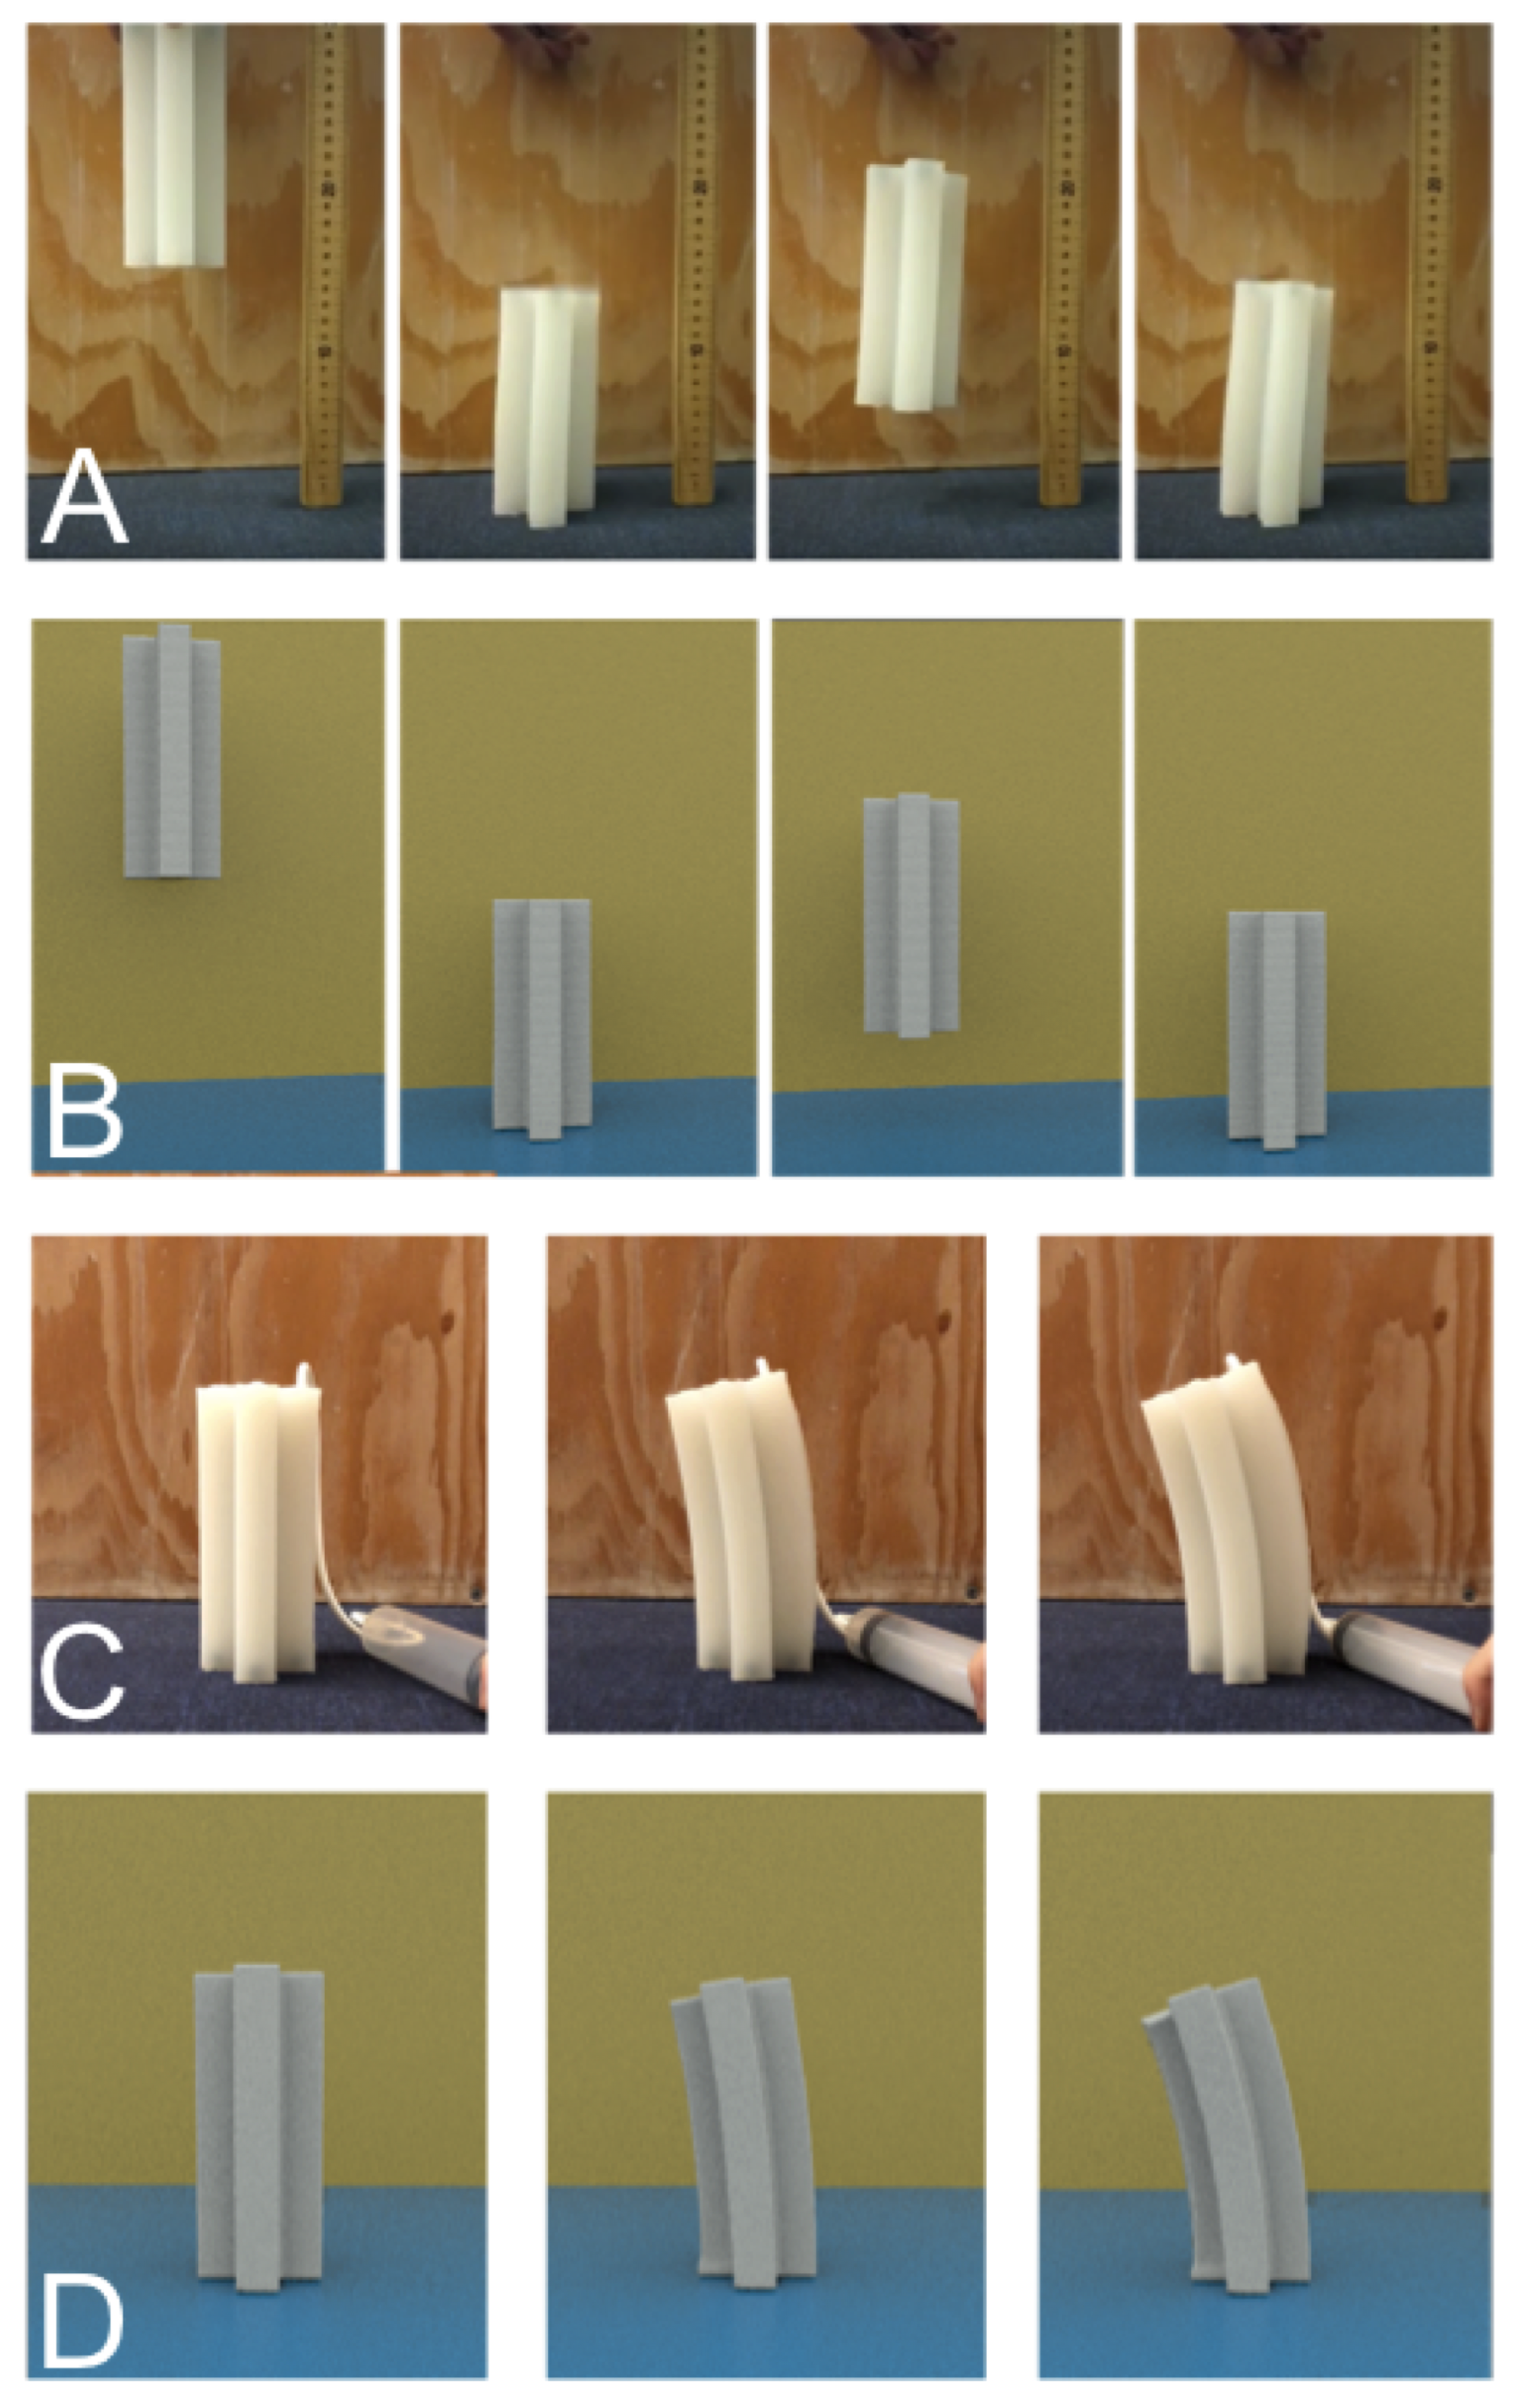
\includegraphics[width=2.5cm]{chain_queen_experiment.png}
  2019 \cite{Hu2019chainqueen}
  \end{center}

  \column{0.21\linewidth}
  \centering
  \begin{center}
  \shadowimage[width=2.5cm]{litlo_paper.png}
  \vspace{0.5cm}
  \shadowimage[width=2.0cm]{litlo_image.png}
  2019 \cite{Spielberg2019}
  \end{center}
\end{columns}
\end{frame}
\placelogotrue

\placelogofalse
\begin{frame}{Applications: Quantized Graphics}
\begin{columns}
  \column{0.48\linewidth}
  \begin{outline}
    \1 Decouple algorithms 
    from data representation
    \1 Lower memory requirements
    \2 8x Game of Life
    \2 1.5x Eulerian Fluid
    \2 1.7x Material point method
    \1 Leads to faster runtimes
  \end{outline}

  \column{0.48\linewidth}
  \centering
  \begin{center}
  \shadowimage[width=3.0cm]{quan_taichi_paper.png}
  2021 \cite{Hu2021} \\
  \vspace{0.3cm}
  \shadowimage[width=4.5cm]{quantized_demo.png}\\
  \end{center}
\end{columns}
\end{frame}
\placelogotrue


\begin{frame}{Interactive Example}
  \begin{center}
    \includegraphics[width=6cm]{julia_set.png}
    \blfootnote{Based on
      \href{https://docs.taichi-lang.org/docs/hello_world}{Hello, World!}
    guide}
  \end{center}
\end{frame}



\begin{frame}{Frontend}
  \begin{center}
    \includegraphics[width=10cm]{taichi_frontend.png}
    \blfootnote{From \href{https://yuanming.taichi.graphics/publication/2020-life-of-kernel/life_of_a_taichi_kernel.pdf}{Life of a Taichi Kernel} slides}
  \end{center}
\end{frame}



\begin{frame}{Life of a Taichi Kernel}
  \begin{center}
    \includegraphics[width=11cm]{life_of_a_taichi_kernel.png}
    \blfootnote{From \href{https://yuanming.taichi.graphics/publication/2020-life-of-kernel/life_of_a_taichi_kernel.pdf}{Life of a Taichi Kernel} slides}
  \end{center}
\end{frame}




\placelogofalse
\begin{frame}{OpenVDB}
\begin{columns}
\column{0.58\linewidth}
\centering
\begin{outline}
    \1 Originally from Dreamworks animation
    \1 Widely used for special effects and animation
      \2 Supported by industry standard software like Houdini and Blender
    \1 Often used with implicit geometry
    \1 Published in ACM Trans. Graphics
    \2 Describes VDB Datastructure
    \2 Introduced OpenVDB implementation
\end{outline}

\column{0.38\linewidth}
\centering
\shadowimage[width=2.5cm]{vdb_paper.png}
2013 \cite{Museth2013}\\
\vspace{0.5cm}
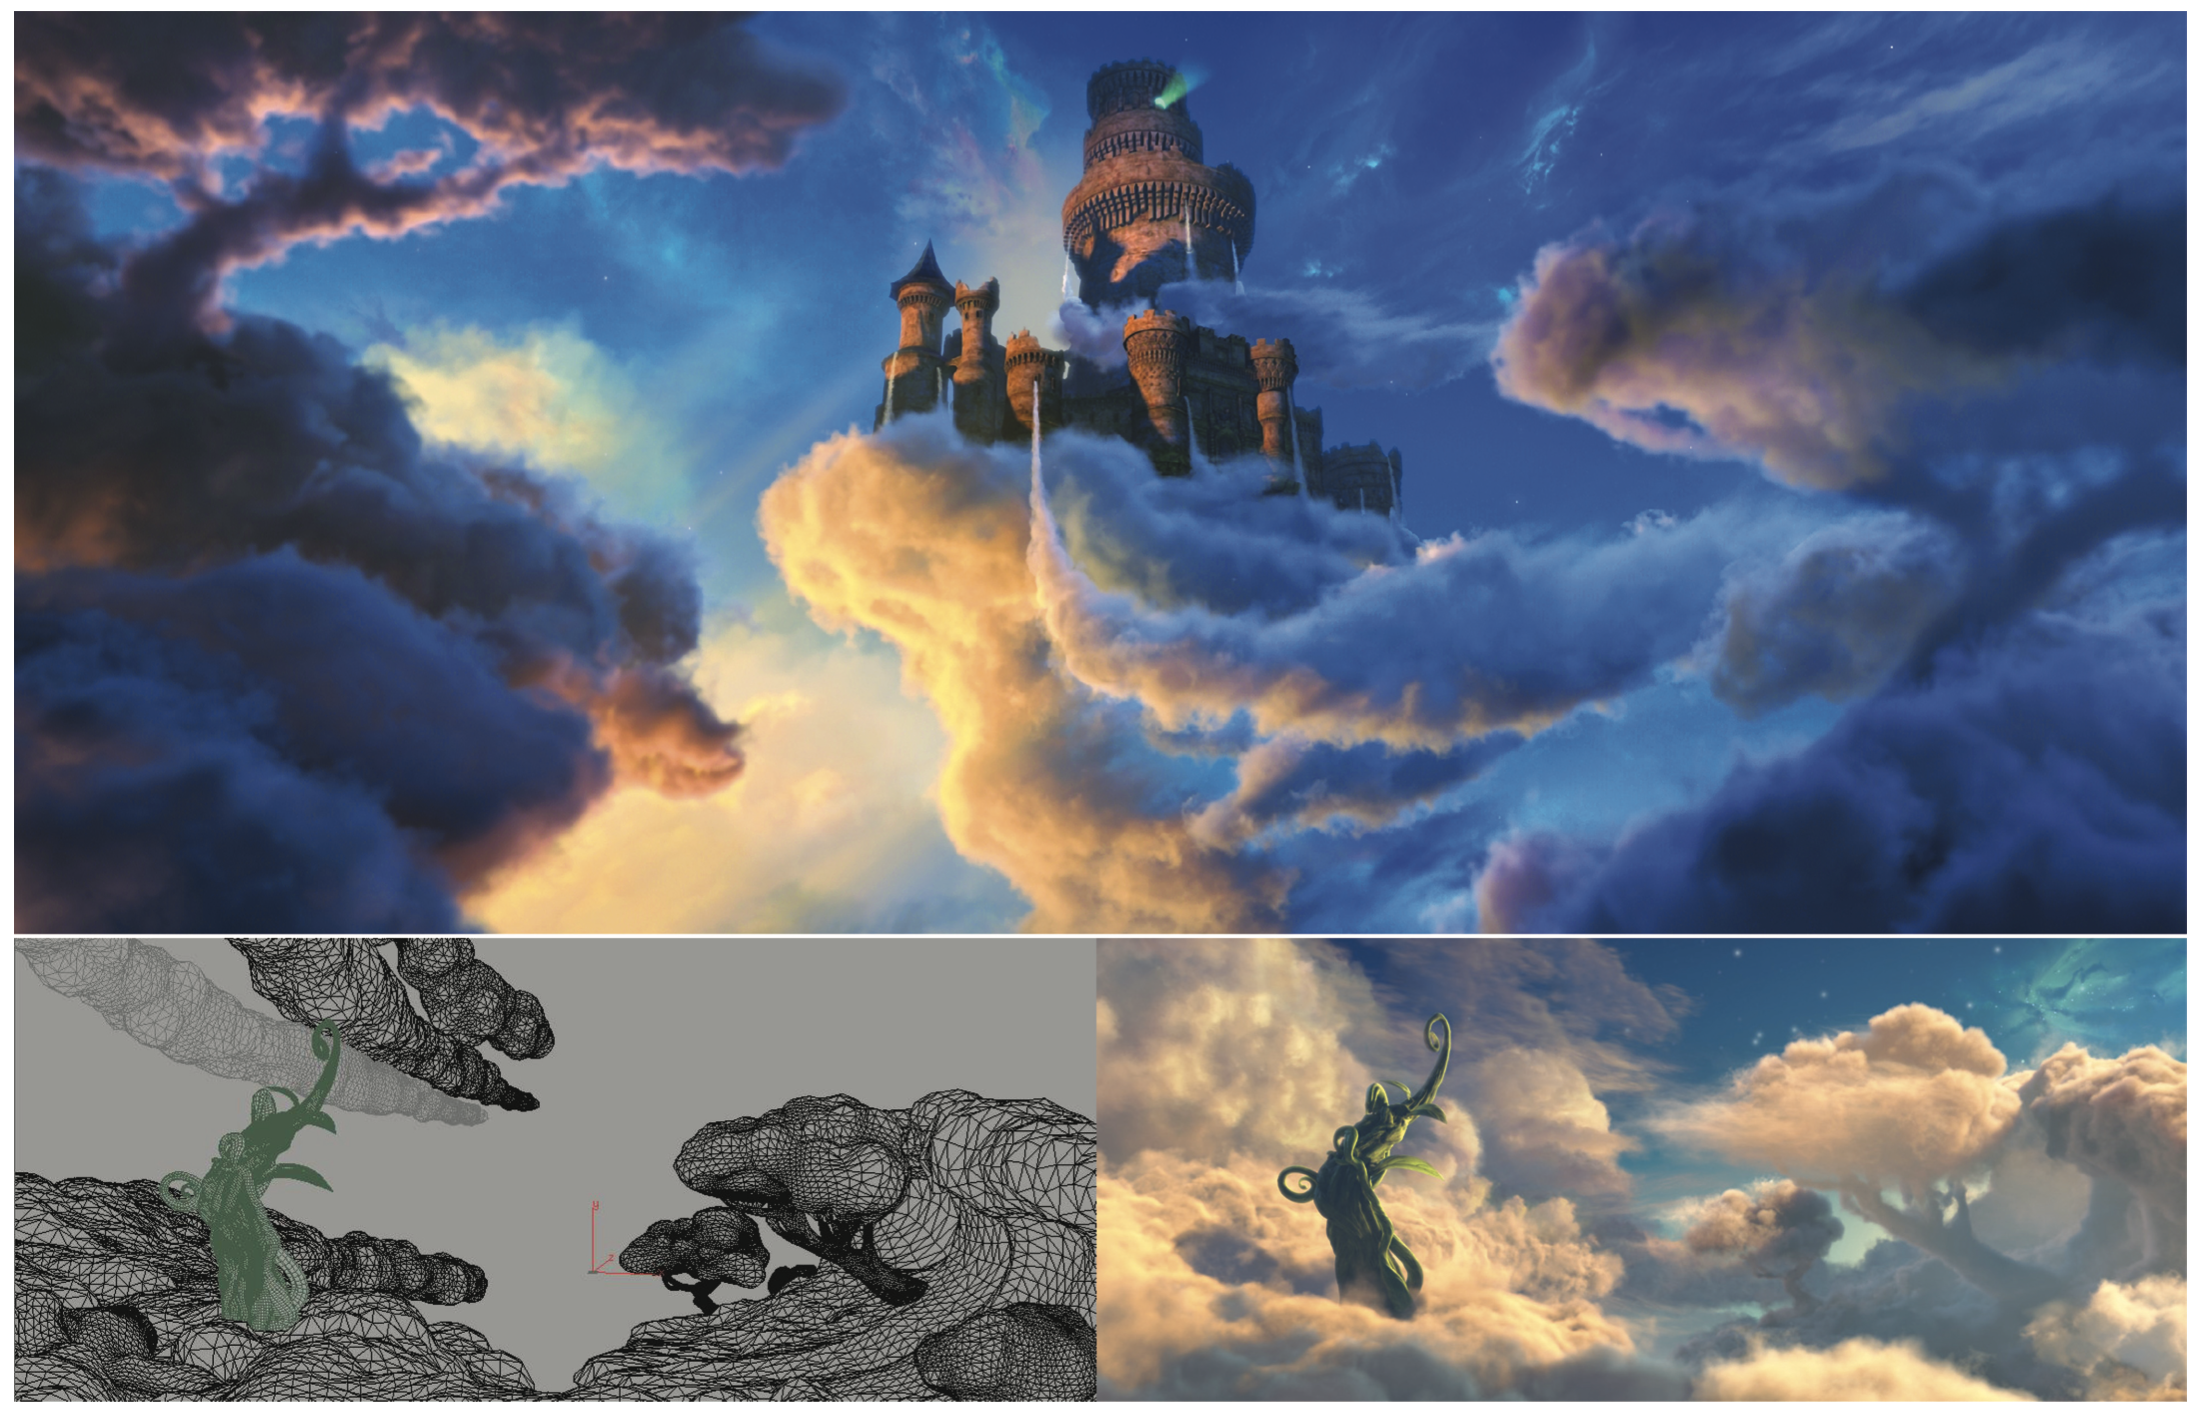
\includegraphics[width=4cm]{open_vdb_puss_in_boots.png} 
\end{columns}
\end{frame}
\placelogotrue

\begin{frame}{VDB Datastructure}
\begin{columns}
\column{0.38\linewidth}
\centering
\begin{outline}
    \1 Similar to B+Trees
    \1 Map based root 
      \2 Dynamic branching factor
      \2 Virtually infinite spatial bounds
    \1 Fixed height
    \1 Large (fixed) branching factors for children
\end{outline}

\column{0.58\linewidth}
\centering
\includegraphics[width=7.0cm]{open_vdb_data_structure.png} \\
\vspace{0.5cm}
\includegraphics[width=7.0cm]{open_vdb_visual_aid.png} 
\end{columns}
\blfootnote{Images from \cite{Museth2013}}
\end{frame}


\begin{frame}{SPGrid}
\begin{columns}
\column{0.58\linewidth}
\begin{outline}
    \1 ACM Trans. Graphics 2014 \cite{Setaluri2014}
    \1 Key ideas
      \2 Large finite grid replaces infinite map
      \2 Morton key as virtual memory address
      \2 Translation Lookahead Buffer (TLB) handles address translation
\end{outline}
\column{0.38\linewidth}
\centering
\shadowimage[width=3.5cm]{sp_grid_paper.png}
\vspace{0.5cm}
\shadowimage[width=3.5cm]{sp_grid_z_order.png} 
\end{columns}
\end{frame}


\begin{frame}[allowframebreaks]{References}
    \tiny
    \printbibliography
\end{frame}

\begin{frame}{Source Files}
\begin{center}
  The source files live on github:\\
  \url{https://github.com/SallySoul/stencil_latex/tree/main/slides/taichi}
\end{center}
\end{frame}

\end{document}


